\documentclass[12pt,oneside]{amsbook}
\usepackage{graphicx}
\usepackage{subfiles}
\usepackage[backend=biber]{biblatex}

\addbibresource{biblio.bib}

\AtEndDocument{%
    \printbibliography
}

%this sets the margins to 1" on all sides -- the amsbook gives giant margins.
\addtolength{\oddsidemargin}{-.875in}
\addtolength{\evensidemargin}{-.875in}
\addtolength{\textwidth}{1.75in}

\addtolength{\topmargin}{-.5in}
\addtolength{\textheight}{1in}


% above is the preamble
%\renewcommand{\baselinestretch}{2} Use this for double-spacing.

\numberwithin{equation}{chapter}
% This numbers the equations within each chapter as 1.1, 1.2, 2.1, etc.
\numberwithin{figure}{chapter}
% This does the same for the figures.

\theoremstyle{plain} % This is the default style.
\newtheorem{thm}{Theorem}[chapter]
\newtheorem{cor}[thm]{Corollary}
\newtheorem{prop}[thm]{Proposition}
\newtheorem{lem}[thm]{Lemma}
% [chapter] causes the above to be numbered within each chapter as 1.1, 1.2, ...
% If you omit [chapter], the numbers will be 1, 2, ...

\theoremstyle{definition}
\newtheorem*{dfn}{Definition}
% The asterisk suppresses the numbering of definitions.

\theoremstyle{remark}
\newtheorem{ex}{Example}
\newtheorem*{rem}{Remark}
% The asterisk suppresses the numbering of remarks.

\graphicspath{{../images/}}

%allows subfiles to reference biblio.bib




\begin{document}





\frontmatter % Pages here will be numbered with Roman numerals.
\title[]{Building a Spectroscopy Apparatus Around the FP4209 InstaTune}
\author{James Usher}
\address{Department of Physics and Astronomy \\Bates College\\Lewiston, ME 04240}
\date{April 1, 2026}
\maketitle

% Create real cover page.
\thispagestyle{empty} 			% Suppress numbering of this page.
\subfile{cover}     			% Save the file cover.tex to the same folder as thesis.tex.
\setcounter{page}{2}

\tableofcontents
% This creates a file called thesis.toc.

% \listoftables
% \listoffigures
% Use the above if you have tables/figures and want them listed in the front.

% The following files should be in the same folder as thesis.tex.
%\include{ack}     			% Acknowledgments
\subfile{acknowledgements.tex}
%\chapter{Introduction}\label{introduction}

\section{Background}

\section{Motivation}


\subsection{Subsection}
 

\subsection{Another subsection} 

\section{Another section}
   			% Introduction 
\subfile{introduction.tex}
\mainmatter % Pages here will be numbered 1, 2, 3, and so on .

% The following files should also be in the same folder as thesis.tex.
\subfile{chapter1.tex}
%\documentclass[../main]{subfiles}

\begin{document}
\chapter{Method}
\section*{Laser Functionality}

\section*{Program Sequencing}

%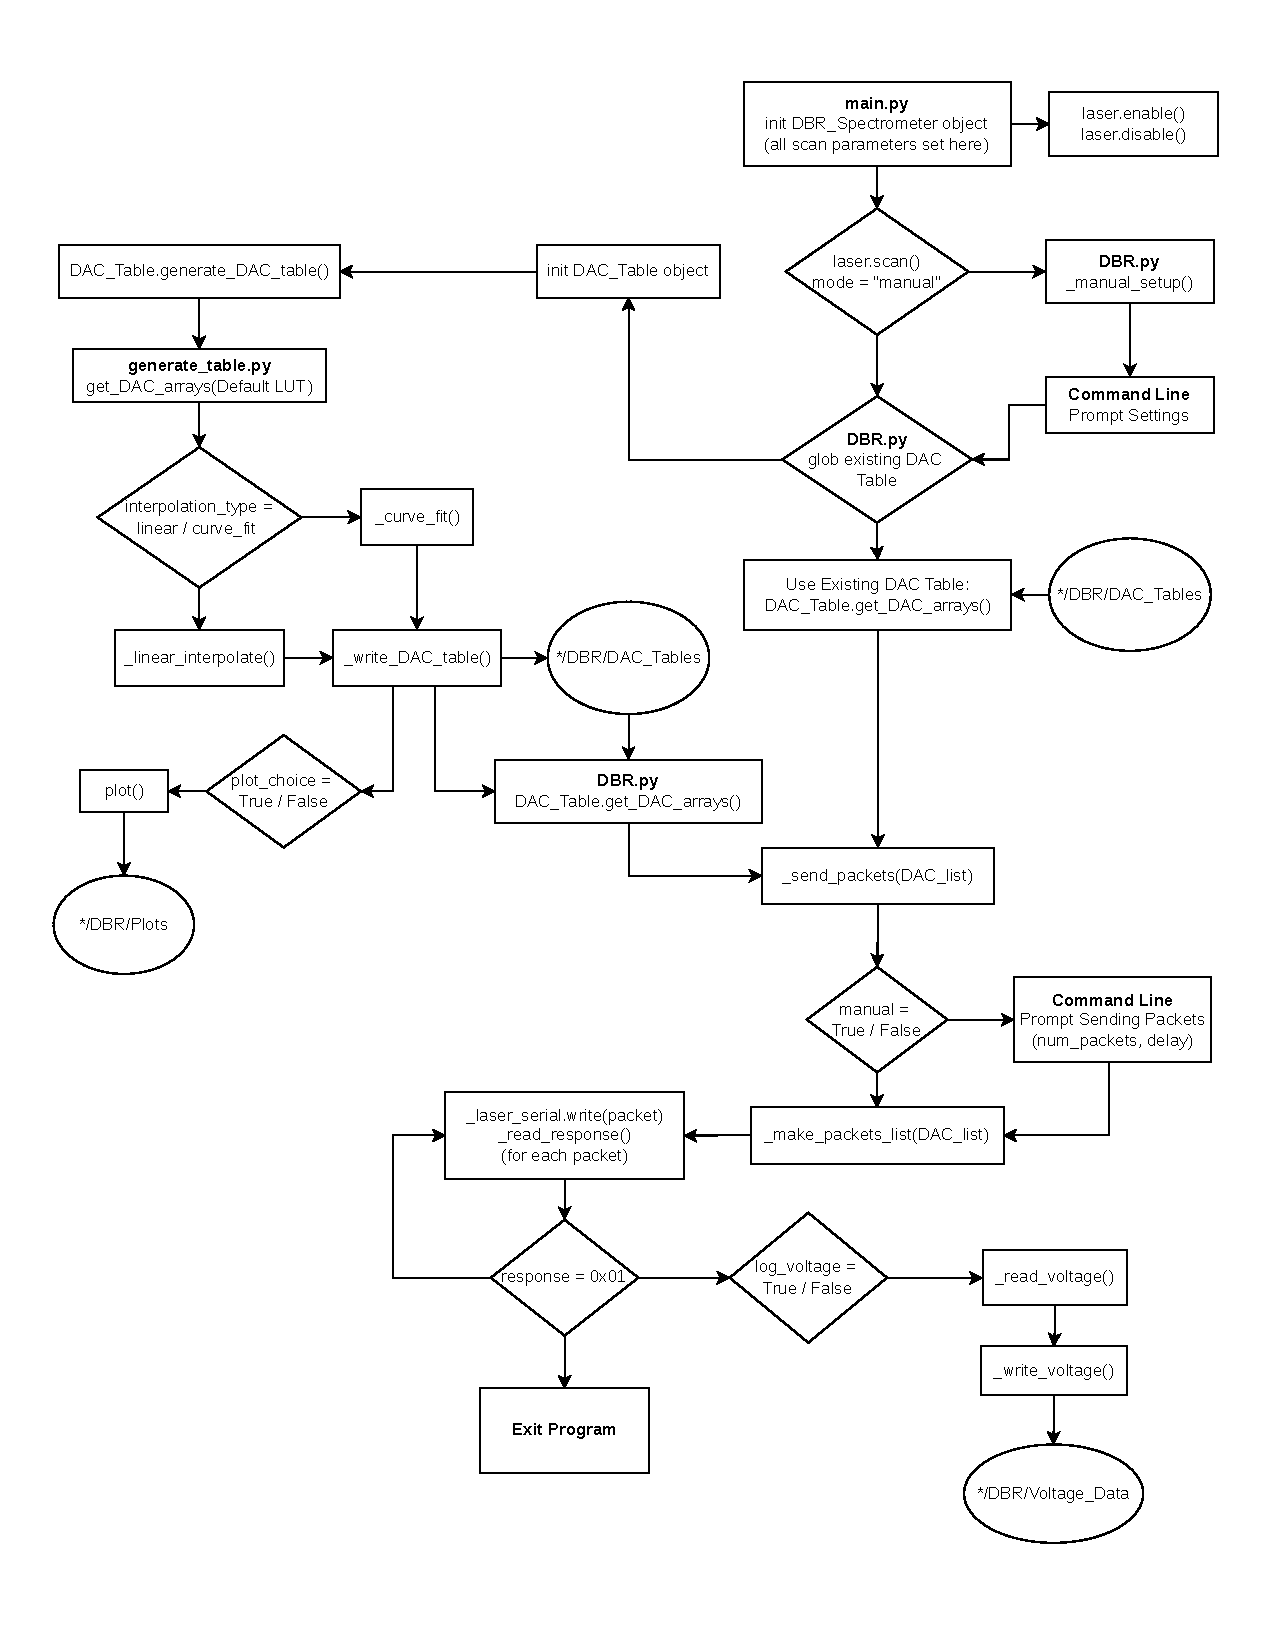
\includegraphics[]{DBR_flowchart.pdf}
\fbox{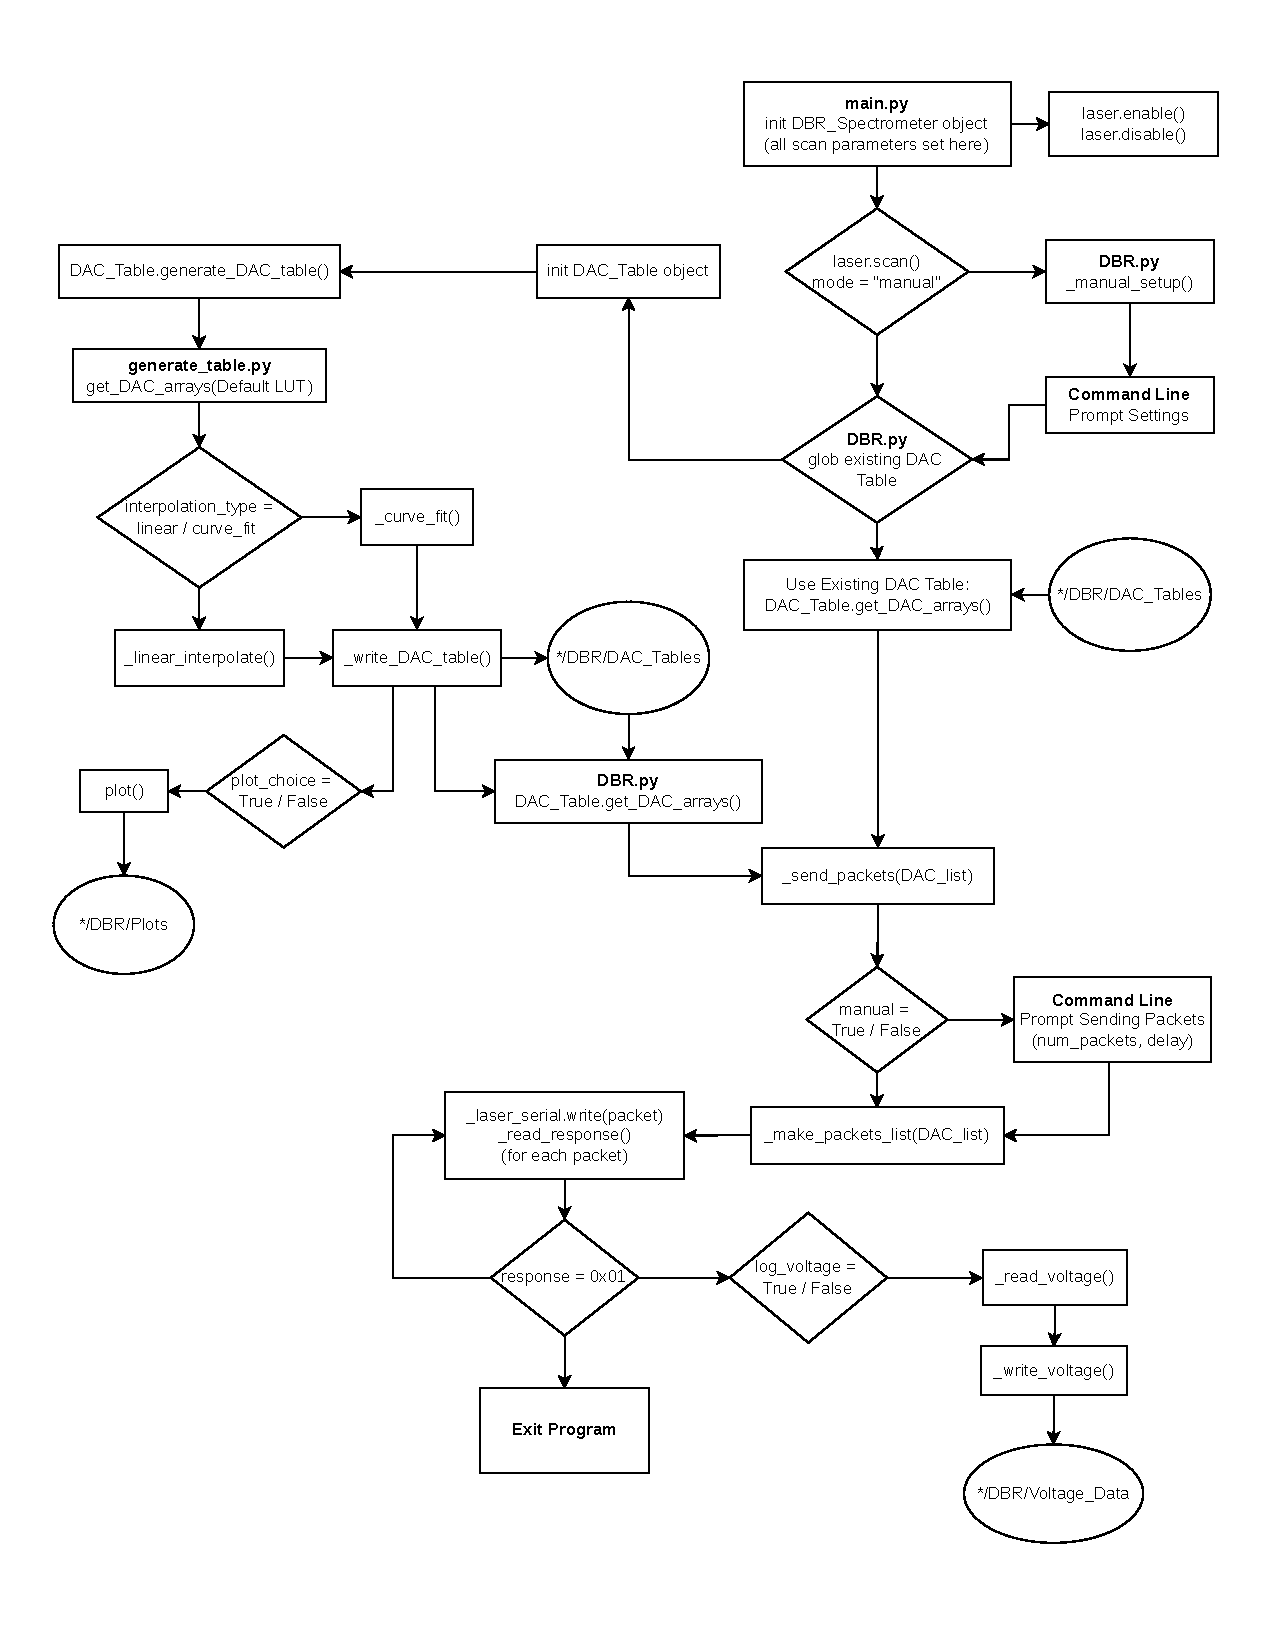
\includegraphics[width=\textwidth]{DBR_flowchart.pdf}}
% Flow Charts and Code timing
\section*{Communication Protocol}

\section*{Data Collection}

wooooo
\end{document} % Use the same command to add more chapters or sections
\subfile{chapter2.tex}

\subfile{chapter3.tex}
\backmatter
%

\documentclass[../main]{subfiles}
\begin{document}
\chapter*{Appendix A}
% The asterisk prevents this file from being labelled
% as a 'chapter.'

Long derivations, marginally relevant details, and the like can be relegated to your appendix, which unlike the mammalian counterpart will never require removal.
\end{document}			% Use \include{appendixB} to include another appendix.
\subfile{appendixA.tex}

\end{document}